\documentclass[11pt,a4paper]{article}
\usepackage[margin=0.85in]{geometry}
\usepackage{graphicx}
\usepackage{booktabs}
\usepackage{array}
\usepackage{amsmath,amssymb}
\usepackage{hyperref}
\usepackage{float}
\usepackage{caption}
\usepackage[table]{xcolor}
\usepackage{enumitem}
\hypersetup{colorlinks=true,linkcolor=blue!50!black,urlcolor=blue!50!black}
\graphicspath{{../results/}}
\setlength{\parskip}{4pt}
\setlength{\parindent}{0pt}

\title{ML-Driven PVT Variation Aware Leakage Estimation}
\author{Digital VLSI Design --- Course Project}
\date{November 2026}

\begin{document}
\maketitle

\noindent Model file \textbf{16nm\_HP}, nominal \textbf{VDD 0.9 V}, test circuit \textbf{3-bit carry-lookahead adder (CLA)}.

\section*{Summary}
\noindent Model file \textbf{16nm\_HP}, nominal \textbf{VDD 0.9 V}, test circuit \textbf{3-bit carry-lookahead adder (CLA)}.\\
Repository: \url{https://github.com/rtvk2/dvd-leakage-estimation}

\begin{table}[H]\centering\small
\caption{Summary of results (relative error against SPICE)}
\resizebox{\textwidth}{!}{%
\begin{tabular}{lccc}\toprule
Level & Median error [\%] & 95th pct [\%] & Mean error [\%]\\\midrule
Transistor currents (4 models, 1{,}500 test samples each) & 0.26 to 1.28 & 1.3 to 11.7 & 0.45 to 3.51\\
Gate leakage (5 gates, 18 cases $\times$ 200 corners = 3{,}600 pts) & 0.58 & 2.37 & 0.83\\
3-bit CLA leakage, hierarchical (128 vectors $\times$ 200 corners = 25{,}600 pts) & 1.50 & 6.15 & 2.07\\
3-bit CLA with perfect gate models (composition floor) & 1.37 & 5.25 & 1.85\\
\bottomrule\end{tabular}}
\end{table}

The $R^2$ of the signed-log currents is at least 0.9996 for every transistor model. The gate-level error is below 3\% for 95\% of the points. The circuit-level hierarchical prediction has mean error 2.07\% (mean accuracy $100\%-2.07\%=97.93\%$, below a 99\% target); this is dominated by the prescribed composition method (ideal 0/VDD inputs, no inter-gate loading), whose oracle/composition floor is 1.37\% median / 5.25\% 95th / 1.85\% mean even with perfect gate models.

\section{Setup}
\begin{table}[H]\centering\small
\caption{Assignment and tools}
\begin{tabular}{p{3.2cm}p{11.4cm}}\toprule
Item & Value\\\midrule
Model file & 16nm\_HP: PTM high-performance 16 nm, metal gate / high-k, BSIM4 (level 54), TNOM 27$^\circ$C\\
Nominal VDD & 0.9 V (file header states 0.7 V; assigned 0.9 V used, so VDD sampled 0.81--0.99 V)\\
Geometry & $L = 16$ nm (= Lmin); $W \in [1\times, 8\times]$Lmin, i.e.\ 16--128 nm\\
Test circuit & 3-bit carry-lookahead adder with carry-in (7 inputs, 128 input vectors)\\
Simulator & ngspice-42, batch mode (\texttt{ngspice -b}) via WSL on Windows 11; \texttt{.options gmin=1e-18 abstol=1e-18 reltol=1e-6 vntol=1e-9} in every netlist; \texttt{set numdgt = 15}\\
Software & Python 3.12.8, numpy 1.26.4, pandas 2.2.3, scikit-learn 1.5.1, LightGBM 4.6.0, PyTorch 2.7.0 (CPU), matplotlib 3.9.2\\
\bottomrule\end{tabular}\end{table}

The work is organised as seven self-contained Jupyter notebooks (\texttt{notebooks/01}--\texttt{07}); numbered scripts \texttt{scripts/01\_gen\_data.py}--\texttt{07\_error\_analysis.py} run the corresponding notebooks in order (or use \texttt{scripts/run\_all.py}) with fixed seeds. They produce datasets (\texttt{data/}), example netlists (\texttt{netlists/}), four saved models (\texttt{models/}) and all tables/plots (\texttt{results/}).

\section{Data Generation}

\subsection{Sampling}
For each of the four cases (NMOS ON, NMOS OFF, PMOS ON, PMOS OFF) 10{,}000 samples were drawn per the project text. VDD is drawn first (uniform, 0.9 V $\pm$ 10\%); then drain and source voltages (uniform in $[0,\mathrm{VDD}]$), width (uniform 16--128 nm), temperature (uniform $-40$ to $125^\circ$C), and five process parameters \texttt{vth0, toxe, ndep, u0, xj} (uniform, nominal $\pm$ 10\%, separately for NMOS and PMOS cards). Gate/body voltages are fixed by case: NMOS ON (VDD,0), NMOS OFF (0,0), PMOS ON (0,VDD), PMOS OFF (VDD,VDD). Every parameter of every sample is drawn independently; seeds are 20261105 + case index.

\begin{table}[H]\centering\small
\caption{Nominal process parameters from the model file}
\begin{tabular}{lcc}\toprule
Parameter & NMOS nominal & PMOS nominal\\\midrule
vth0 [V] & 0.47965 & $-0.43121$\\
toxe [m] & $9.5\times10^{-10}$ & $1.0\times10^{-9}$\\
ndep [1/cm$^3$] & $7.0\times10^{18}$ & $5.5\times10^{18}$\\
u0 [m$^2$/Vs] & 0.030 & 0.006\\
xj [m] & $5.0\times10^{-9}$ & $5.0\times10^{-9}$\\
\bottomrule\end{tabular}\end{table}

\subsection{Netlists and Simulation}
Each sample is simulated in a one-transistor netlist with its own voltage source on every terminal (\texttt{Vd,Vg,Vs,Vb}); terminal currents flowing into the device are negatives of source currents. Junction areas are set explicitly as $\mathrm{AD}=\mathrm{AS}=W\times 32$ nm. Process parameters are set per sample with \texttt{altermod} (one parameter per line), temperature with \texttt{set temp}, voltages/width/areas with \texttt{alter}, and an operating point (\texttt{op}) is run. 250 samples per ngspice script, scripts run in parallel. No operating-point failures occurred. Example netlists: \texttt{netlists/single\_<case>.cir}.

\subsection{Data Check}
\begin{table}[H]\centering\small
\caption{Kirchhoff check: four terminal currents of every sample sum to zero}
\begin{tabular}{lrrrc}\toprule
Case & Rows & max $|\sum I|$ [A] & median [A] & Passes\\\midrule
NMOS ON & 10{,}000 & $1.55\times10^{-15}$ & $8.99\times10^{-17}$ & yes\\
NMOS OFF & 10{,}000 & $8.49\times10^{-19}$ & $4.80\times10^{-23}$ & yes\\
PMOS ON & 10{,}000 & $9.84\times10^{-16}$ & $3.24\times10^{-17}$ & yes\\
PMOS OFF & 10{,}000 & $1.30\times10^{-15}$ & $8.08\times10^{-17}$ & yes\\
\bottomrule\end{tabular}\end{table}

Residuals are at solver-tolerance level. Trend checks (all Spearman correlations have expected sign):

\begin{table}[H]\centering\small
\caption{Trend checks}
\begin{tabular}{llccc}\toprule
Case & Relation & Spearman & Expected sign & As expected\\\midrule
NMOS OFF & temperature & $+0.235$ & $+$ & yes\\
NMOS OFF & $|v_{th0}|$ & $-0.218$ & $-$ & yes\\
PMOS OFF & temperature & $+0.297$ & $+$ & yes\\
PMOS OFF & $|v_{th0}|$ & $-0.153$ & $-$ & yes\\
NMOS ON & toxe $\to |I_g|$ & $-0.399$ & $-$ & yes\\
NMOS OFF & toxe $\to |I_g|$ & $-0.597$ & $-$ & yes\\
PMOS ON & toxe $\to |I_g|$ & $-0.184$ & $-$ & yes\\
PMOS OFF & toxe $\to |I_g|$ & $-0.683$ & $-$ & yes\\
\bottomrule\end{tabular}\end{table}

\begin{figure}[H]\centering
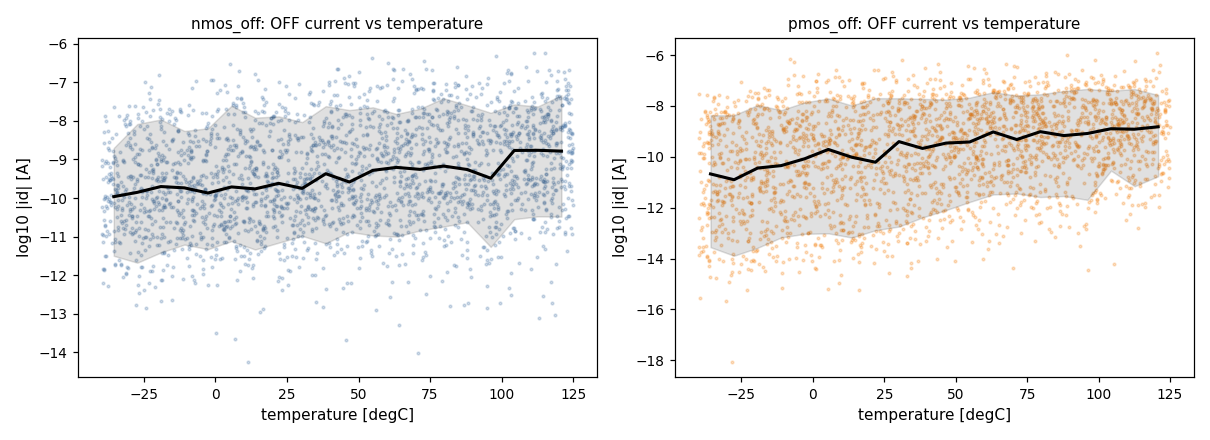
\includegraphics[width=0.7\textwidth]{trend_off_vs_temp.png}
\caption{OFF-state leakage current vs temperature.}\end{figure}
\begin{figure}[H]\centering
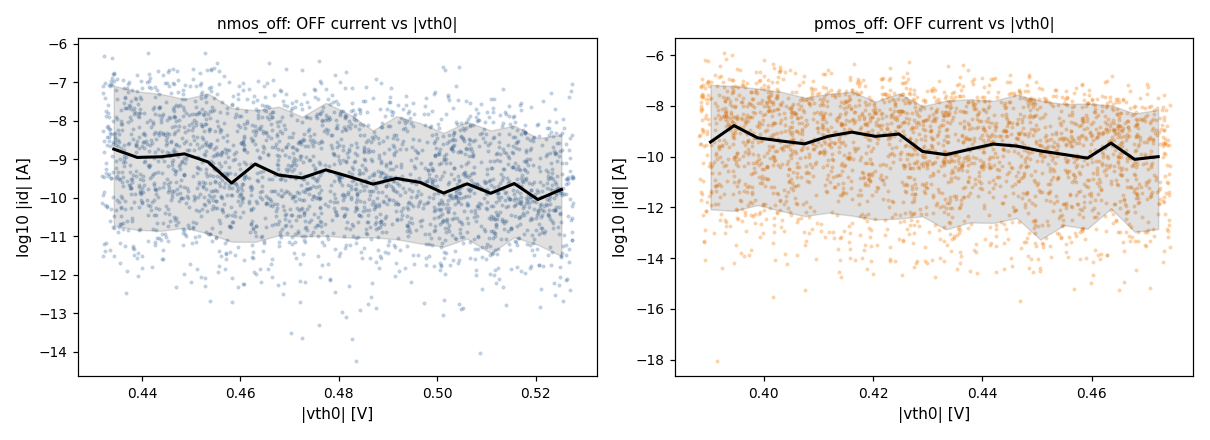
\includegraphics[width=0.7\textwidth]{trend_off_vs_vth0.png}
\caption{OFF-state leakage current vs $|v_{th0}|$.}\end{figure}
\begin{figure}[H]\centering
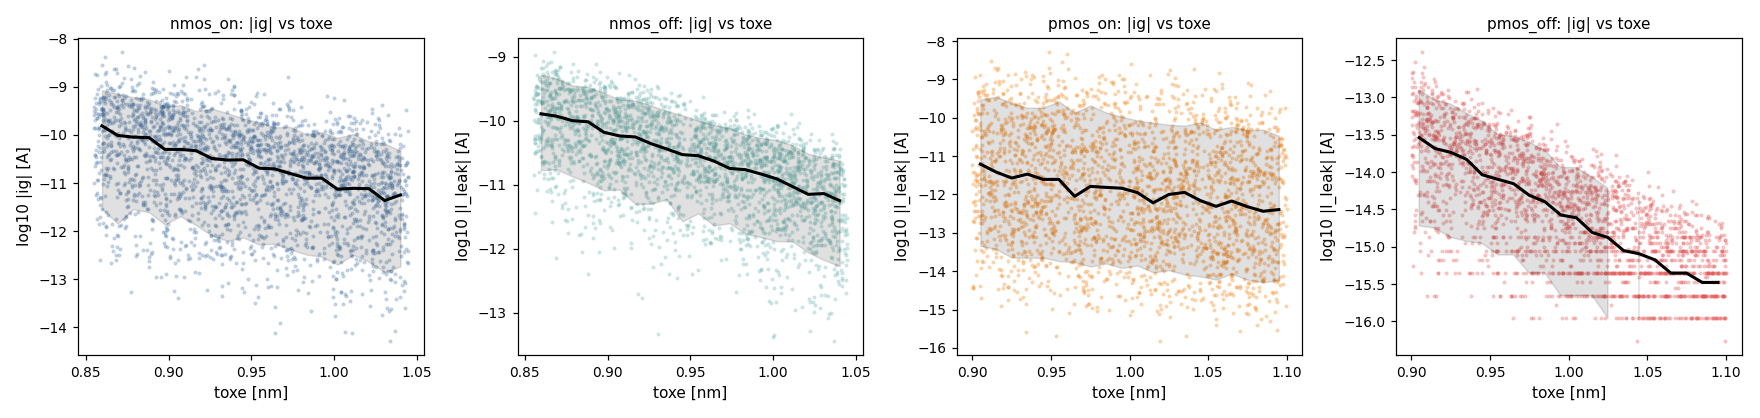
\includegraphics[width=0.7\textwidth]{trend_ig_vs_toxe.png}
\caption{Gate current vs oxide thickness.}\end{figure}

\subsection{Split}
Each dataset is split randomly into 70\% training (7{,}000), 15\% validation (1{,}500) and 15\% test (1{,}500) with fixed seed 20261105. The same split is used for every model type. All choices are made on training/validation; test samples are used once for final chosen models.

\section{Transistor Models}

\subsection{Preprocessing}
\begin{itemize}[leftmargin=*]
\item \textbf{Source/drain canonicalisation.} Each sample mapped to one orientation ($V_{ds}\ge 0$ for NMOS, $V_{sd}\ge 0$ for PMOS; $I_d,I_s$ swap with terminals), fixing signs and removing sign change at $V_d=V_s$. Saved models swap back.
\item \textbf{Target transform.} Models predict $\operatorname{arcsinh}(I/I_0)$ with $I_0=10^{-14}$ A (chosen on validation; preserves sign, relative scale for large currents, linear near zero).
\item \textbf{Vds-aware target (option).} For $I_d,I_s$, divide by $(1-\exp(-V_{ds}/V_T))$ before transform (chosen per case on validation) to smooth behavior at very small $|V_{ds}|$.
\item \textbf{Features.} 12 raw inputs plus 8 physics features: $q/kT$, $V_{gs}$, $V_{ds}$, $V_{bs}$, $V_{gd}$, $(V_{gs}-v_{th0})/V_T$, $V_{ds}/V_T$, $\ln W$ (source-referenced, sign-mirrored for PMOS). Inputs/targets standardised using training-set statistics only.
\end{itemize}

\subsection{Model Types and Hyperparameters}
One model per case, each predicting $I_d,I_g,I_s,I_b$. Four model types compared:

\begin{table}[H]\centering\small
\caption{Model types}
\resizebox{\textwidth}{!}{%
\begin{tabular}{p{3.2cm}p{11.5cm}}\toprule
Model type & Main hyperparameters\\\midrule
Polynomial ridge regression & Polynomial features of standardised inputs (degrees 2--4 on 12 raw inputs, 2--3 on 20 physics features, $\le\sim$1800 terms); ridge penalty chosen per target by LOO-CV on training samples\\
Gradient boosting (LightGBM) & One regressor per current, 31 leaves, LR 0.05, up to 3{,}000 trees with early stopping on validation, row/column subsampling 0.8/0.9, deterministic\\
MLP & 3 hidden layers $\times$ 256 units, SiLU; AdamW (wd $10^{-5}$), batch 256, one-cycle LR (peak $3\times10^{-3}$), 600 epochs, seed 0; best validation epoch kept\\
Residual MLP (ResNN) & Input 128, 4 residual blocks $h \leftarrow \mathrm{SiLU}(h + \mathrm{Linear}(\mathrm{SiLU}(\mathrm{Linear}(h))))$, linear output; same training as MLP\\
\bottomrule\end{tabular}}
\end{table}

For each model type/case, option sets (raw/physics features, Vds-aware on/off, and for networks MSE/Huber loss) were compared on validation. \textbf{Selection rule:} lowest mean over four currents of median relative error $|pred-true|/|true|$ (rows with $|I|\ge10^{-15}$ A).

\subsection{Model Comparison on Validation Set}
\begin{table}[H]\centering\scriptsize
\caption{Validation set: per-model-type $R^2$ (signed-log), median and 95th-percentile relative error (mean over four currents)}
\resizebox{\textwidth}{!}{%
\begin{tabular}{lccc ccc ccc ccc}\toprule
 & \multicolumn{3}{c}{Poly.\ ridge} & \multicolumn{3}{c}{LightGBM} & \multicolumn{3}{c}{MLP} & \multicolumn{3}{c}{Residual MLP}\\
\cmidrule(lr){2-4}\cmidrule(lr){5-7}\cmidrule(lr){8-10}\cmidrule(lr){11-13}
Case & $R^2$ & Med\% & P95\% & $R^2$ & Med\% & P95\% & $R^2$ & Med\% & P95\% & $R^2$ & Med\% & P95\%\\\midrule
NMOS ON  & 0.9980 & 7.06 & 27.7 & 0.9983 & 5.90 & 27.8 & 1.0000 & 0.54 & 3.25 & 1.0000 & 0.39 & 2.17\\
NMOS OFF & 0.9736 & 33.43 & 268.9 & 0.9941 & 7.56 & 39.6 & 0.9987 & 0.86 & 8.59 & 0.9995 & 0.59 & 4.13\\
PMOS ON  & 0.9983 & 8.26 & 31.1 & 0.9981 & 7.62 & 31.9 & 1.0000 & 0.36 & 1.90 & 1.0000 & 0.24 & 1.24\\
PMOS OFF & 0.9875 & 25.58 & 175.8 & 0.9975 & 8.87 & 38.5 & 0.9995 & 1.67 & 14.18 & 0.9996 & 1.24 & 9.85\\
\bottomrule\end{tabular}}
\end{table}

\begin{figure}[H]\centering
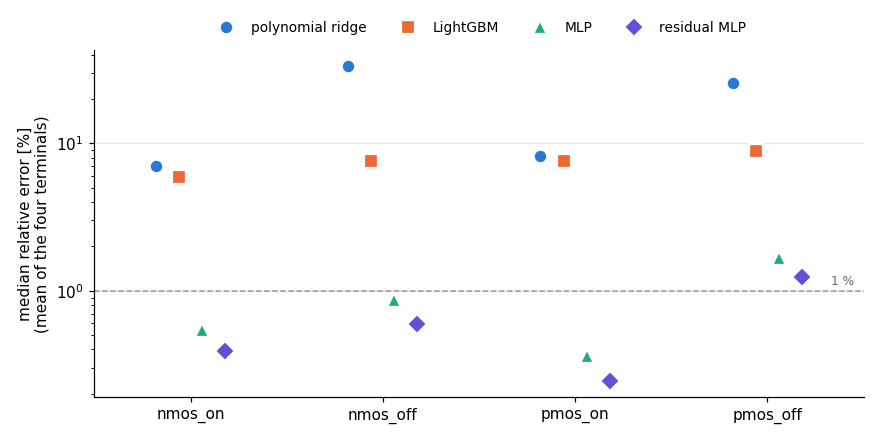
\includegraphics[width=0.7\textwidth]{model_comparison.png}
\caption{Median relative error of the four model types (validation set, log axis).}\end{figure}

\textbf{Final choice.} Residual MLP is best on validation for all four cases (7--31$\times$ lower median error than best classical model; 1.35--1.5$\times$ lower than plain MLP). Final models: NMOS ON/PMOS ON with Vds-aware target + Huber, NMOS OFF without Vds-aware (MSE), PMOS OFF with Vds-aware (MSE), all with physics features and 600 epochs.

\subsection{Final Models on Test Set}
\begin{table}[H]\centering\small
\caption{Final models, test set (1{,}500 samples per case; errors mean over four currents)}
\resizebox{\textwidth}{!}{%
\begin{tabular}{llccccc}\toprule
Case & Version & Val med [\%] & Test med [\%] & Test p95 [\%] & Test mean [\%] & Test $R^2$ (log)\\\midrule
NMOS ON  & as chosen & 0.39 & 0.37 & 2.19 & 0.73 & 1.0000\\
NMOS OFF & refined (rail samples) & 0.74 & 0.69 & 4.64 & 1.62 & 0.9996\\
PMOS ON  & as chosen & 0.24 & 0.26 & 1.31 & 0.45 & 1.0000\\
PMOS OFF & refined (rail samples) & 1.29 & 1.28 & 11.68 & 3.51 & 0.9996\\
\bottomrule\end{tabular}}
\end{table}

\begin{table}[H]\centering\scriptsize
\caption{Final models, test set, per current}
\begin{tabular}{llrrrr}\toprule
Case & Current & Median [\%] & 95th pct [\%] & Mean [\%] & Median, $|V_{ds}|<5$mV [\%]\\\midrule
NMOS ON  & $I_d$ & 0.40 & 2.47 & 0.83 & 1.22\\
NMOS ON  & $I_g$ & 0.36 & 1.97 & 0.65 & 0.72\\
NMOS ON  & $I_s$ & 0.37 & 2.20 & 0.76 & 0.93\\
NMOS ON  & $I_b$ & 0.36 & 2.10 & 0.69 & 0.61\\
NMOS OFF & $I_d$ & 0.47 & 2.63 & 0.94 & 0.52\\
NMOS OFF & $I_g$ & 0.36 & 1.95 & 0.61 & 0.33\\
NMOS OFF & $I_s$ & 1.09 & 9.67 & 3.59 & 0.75\\
NMOS OFF & $I_b$ & 0.84 & 4.29 & 1.34 & 0.88\\
PMOS ON  & $I_d$ & 0.28 & 1.25 & 0.43 & 0.85\\
PMOS ON  & $I_g$ & 0.23 & 1.28 & 0.51 & 0.55\\
PMOS ON  & $I_s$ & 0.28 & 1.16 & 0.42 & 0.56\\
PMOS ON  & $I_b$ & 0.23 & 1.55 & 0.46 & 0.58\\
PMOS OFF & $I_d$ & 1.31 & 10.12 & 3.46 & 26.52\\
PMOS OFF & $I_g$ & 1.35 & 16.07 & 4.09 & 1.14\\
PMOS OFF & $I_s$ & 1.56 & 15.35 & 4.86 & 34.64\\
PMOS OFF & $I_b$ & 0.91 & 5.18 & 1.63 & 1.47\\
\bottomrule\end{tabular}\end{table}

\begin{figure}[H]\centering
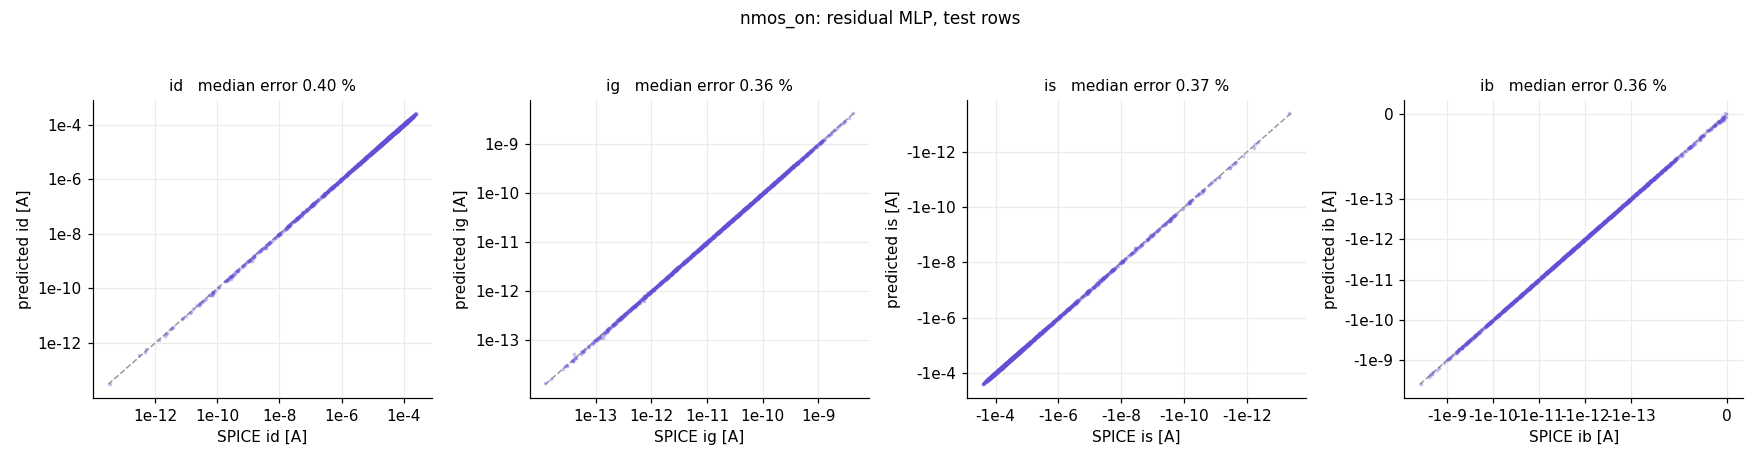
\includegraphics[width=0.85\textwidth]{pred_vs_spice_nmos_on.png}
\caption{Predicted vs SPICE currents, NMOS ON.}\end{figure}
\begin{figure}[H]\centering
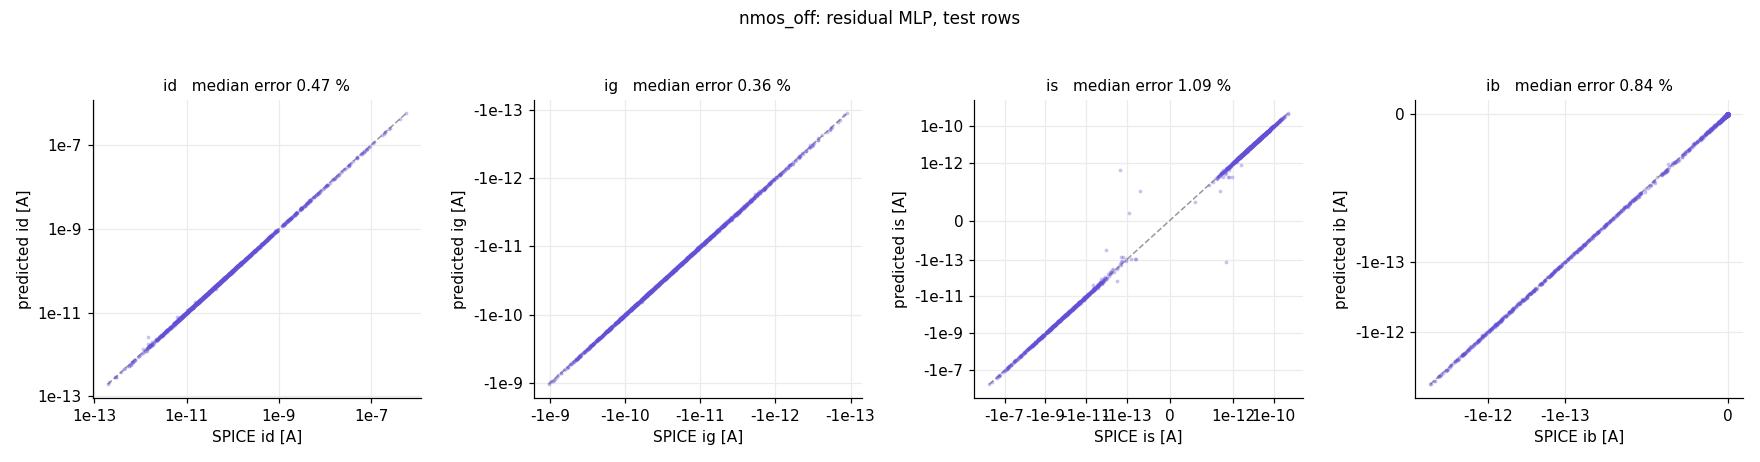
\includegraphics[width=0.85\textwidth]{pred_vs_spice_nmos_off.png}
\caption{Predicted vs SPICE currents, NMOS OFF.}\end{figure}
\begin{figure}[H]\centering
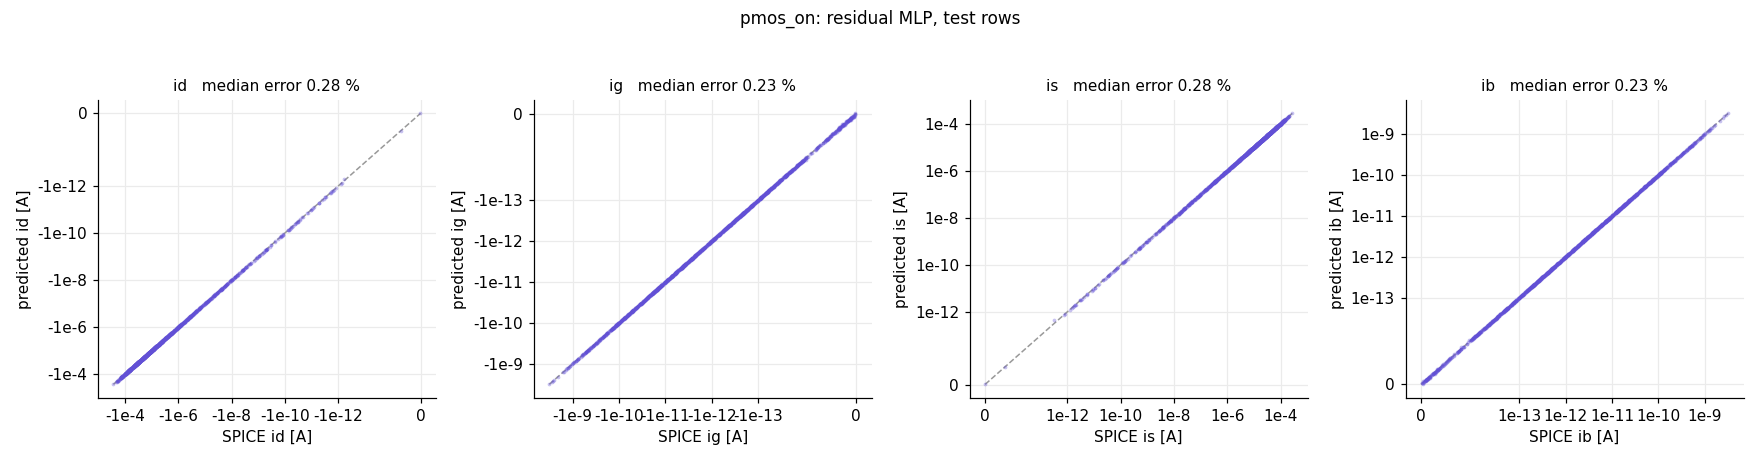
\includegraphics[width=0.85\textwidth]{pred_vs_spice_pmos_on.png}
\caption{Predicted vs SPICE currents, PMOS ON.}\end{figure}
\begin{figure}[H]\centering
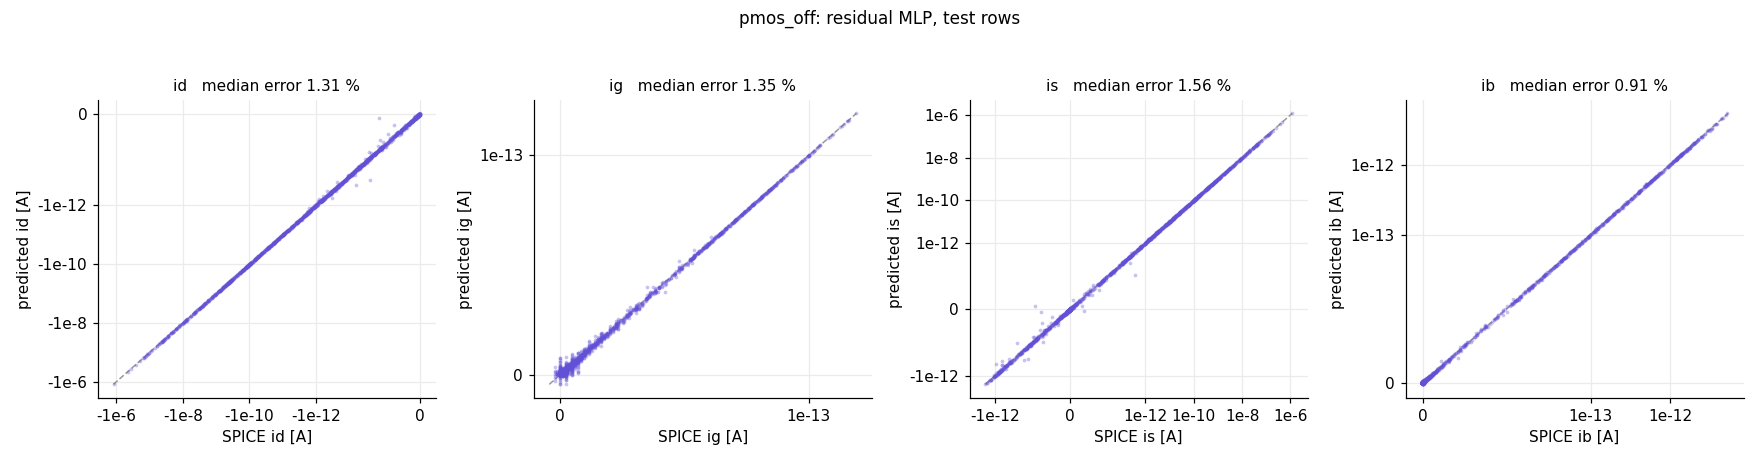
\includegraphics[width=0.85\textwidth]{pred_vs_spice_pmos_off.png}
\caption{Predicted vs SPICE currents, PMOS OFF.}\end{figure}

Test errors agree with validation (max difference $\le 0.05$ pp). Median test error is below 1\% for NMOS ON (0.37\%), NMOS OFF (0.69\%), and PMOS ON (0.26\%); \textbf{PMOS OFF is 1.28\%}. Signed-log $R^2 \ge 0.9996$ for all cases. Hardest currents are PMOS OFF $I_s/I_g/I_d$ (small, sign-sensitive components). At $|V_{ds}|<5$ mV PMOS OFF channel currents have large relative error on few samples, but limited gate-level impact because channel terms are weighted by $V_{ds}$.

\subsection{Rail-Sample Refinement (OFF models) --- Disclosure}
After gate-level analysis showed OFF-model errors concentrate near supply rails, 6{,}000 extra SPICE samples per OFF case were generated (\texttt{data/extra\_nmos\_off.csv}, \texttt{data/extra\_pmos\_off.csv}; no overlap with original 10k datasets) with $V_d,V_s$ biased near rails/uniform mixture (no gate-level simulation/data used). For each OFF case, 5{,}000 extra samples were added to training only and 1{,}000 held out as a separate rail-validation set (not the uniform validation/test sets). Epoch/adoption decisions used uniform+rail validation only; original uniform test sets were used once for reporting. \textbf{No gate or circuit SPICE/ML results were used for training, selection, or tuning.} Adoption rule (validation-only): replace chosen OFF model if rail-validation median and 95th-percentile improve and uniform-validation median rises by $<0.5$ pp. Adopted refined models replaced only the two OFF saved models.

\section{Gate-Level Validation}

\subsection{Gates, Corners, and SPICE Reference}
Gates: INV (A=0,1), NAND2/NOR2/AND2/OR2 (AB=00,01,10,11) = 18 cases $\times$ 200 PVT corners = 3{,}600 SPICE simulations. Static CMOS; AND2=NAND2+INV, OR2=NOR2+INV as full netlists. \textbf{Corner draws:} each corner is one draw with \textbf{VDD and temperature common} to the gate/circuit; the five process parameters ($v_{th0},t_{oxe},ndep,u_0,x_j$) are drawn \textbf{separately for NMOS and PMOS} model cards from the Section~2.1 distributions (all NMOS devices in a gate/circuit share the NMOS draw, all PMOS share the PMOS draw). Corners are drawn once with fixed seed and stored in \texttt{data/corners.csv} (columns \texttt{corner,vdd,temp,n\_*,p\_*}) and reused for gates and test circuit. Inputs are exactly 0 or VDD. SPICE records leakage, internal/output node voltages. ML takes recorded node voltages to set each transistor's $(V_d,V_g,V_s,V_b)$, applies the 4 trained transistor models, and sums predicted currents into gate leakage.

Gate sizing: XX=2, $W_{min}=16$ nm, $L_{min}=16$ nm, $L_{diff}=32$ nm.

\subsection{Gate Results}
\begin{table}[H]\centering\scriptsize
\caption{Gate results, 200 corners per case (bias = mean signed relative error $(ML-SPICE)/SPICE$)}
\resizebox{\textwidth}{!}{%
\begin{tabular}{llcccccc}\toprule
Gate & Input & SPICE med [A] & ML med [A] & Bias [\%] & Med err [\%] & P95 err [\%] & Mean err [\%]\\\midrule
INV   & 0  & $6.50\times10^{-8}$ & $6.53\times10^{-8}$ & $-0.38$ & 0.47 & 1.97 & 0.69\\
INV   & 1  & $3.00\times10^{-7}$ & $2.98\times10^{-7}$ & $+0.36$ & 0.60 & 2.58 & 0.87\\
NAND2 & 00 & $8.74\times10^{-10}$ & $8.74\times10^{-10}$ & $+0.21$ & 0.47 & 1.58 & 0.58\\
NAND2 & 01 & $1.56\times10^{-7}$ & $1.56\times10^{-7}$ & $+0.27$ & 0.35 & 1.54 & 0.49\\
NAND2 & 10 & $2.28\times10^{-8}$ & $2.29\times10^{-8}$ & $+0.36$ & 0.52 & 2.24 & 0.72\\
NAND2 & 11 & $5.86\times10^{-7}$ & $5.83\times10^{-7}$ & $+0.35$ & 0.60 & 2.50 & 0.85\\
NOR2  & 00 & $1.30\times10^{-7}$ & $1.30\times10^{-7}$ & $-0.38$ & 0.48 & 1.96 & 0.68\\
NOR2  & 01 & $5.98\times10^{-7}$ & $5.95\times10^{-7}$ & $+0.45$ & 0.79 & 2.85 & 1.04\\
NOR2  & 10 & $5.38\times10^{-8}$ & $5.37\times10^{-8}$ & $-0.03$ & 0.64 & 1.91 & 0.77\\
NOR2  & 11 & $9.40\times10^{-10}$ & $9.43\times10^{-10}$ & $+0.10$ & 0.69 & 2.17 & 0.83\\
AND2  & 00 & $3.01\times10^{-7}$ & $3.00\times10^{-7}$ & $+0.35$ & 0.59 & 2.58 & 0.86\\
AND2  & 01 & $5.12\times10^{-7}$ & $5.11\times10^{-7}$ & $-0.93$ & 0.90 & 3.63 & 1.29\\
AND2  & 10 & $3.26\times10^{-7}$ & $3.27\times10^{-7}$ & $+0.01$ & 0.58 & 2.52 & 0.82\\
AND2  & 11 & $6.63\times10^{-7}$ & $6.63\times10^{-7}$ & $-0.28$ & 0.66 & 2.62 & 0.86\\
OR2   & 00 & $4.85\times10^{-7}$ & $4.91\times10^{-7}$ & $-0.93$ & 0.89 & 3.81 & 1.27\\
OR2   & 01 & $6.66\times10^{-7}$ & $6.72\times10^{-7}$ & $-0.24$ & 0.71 & 2.83 & 1.01\\
OR2   & 10 & $1.34\times10^{-7}$ & $1.33\times10^{-7}$ & $-0.47$ & 0.47 & 1.83 & 0.67\\
OR2   & 11 & $6.58\times10^{-8}$ & $6.61\times10^{-8}$ & $-0.38$ & 0.49 & 1.94 & 0.67\\
\bottomrule\end{tabular}}
\end{table}

Over all 3{,}600 points: \textbf{median 0.58\%}, 95th percentile 2.37\%, mean 0.83\% (bias $-0.09$\%, max 8.40\%). Best: NAND2 01 (0.35\%); worst: AND2 01 and OR2 00 (internal inverter driven by non-rail node).

\begin{figure}[H]\centering
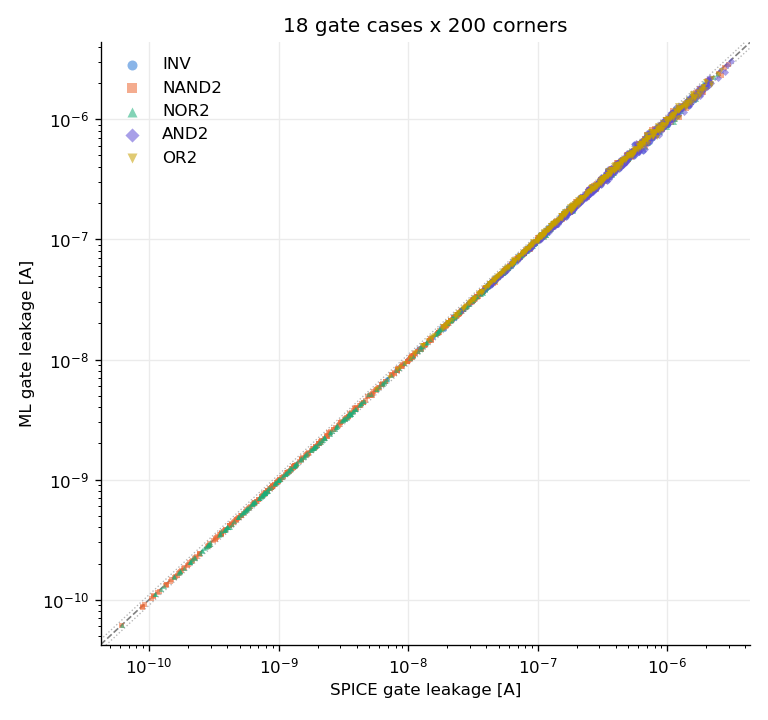
\includegraphics[width=0.65\textwidth]{gate_parity.png}
\caption{ML vs SPICE gate leakage, 18 cases $\times$ 200 corners (log axes).}\end{figure}

\begin{table}[H]\centering\small
\caption{Gate-level error progression (sizing/refinement decisions)}
\begin{tabular}{lccccc}\toprule
Version & Median [\%] & P95 [\%] & Mean [\%] & Bias [\%] & Max [\%]\\\midrule
XX=1 sizing, first OFF models & 2.01 & 8.45 & 2.82 & $-1.17$ & 18.03\\
XX=2 sizing, first OFF models & 1.49 & 7.36 & 2.34 & $-0.75$ & 16.47\\
XX=2 sizing, refined OFF models (final) & 0.58 & 2.37 & 0.83 & $-0.09$ & 8.40\\
\bottomrule\end{tabular}\end{table}

\section{Test Circuit: 3-bit Carry-Lookahead Adder}

\subsection{Circuit and Method}
3-bit CLA with carry-in, built from the five gate types: generate $g_i=a_i b_i$, propagate $p_i=a_i\oplus b_i$, $c_1=g_0+p_0c_0$, $c_2=g_1+p_1g_0+p_1p_0c_0$, $c_3=g_2+p_2g_1+p_2p_1g_0+p_2p_1p_0c_0$, $s_i=p_i\oplus c_i$. XOR = 4 NAND2 gates; products as AND2 (shared sub-products reused); sums as OR2. \textbf{40 gates (24 NAND2, 10 AND2, 6 OR2; 192 transistors)}, 7 inputs ($a_0..a_2,b_0..b_2,c_0$ $\to$ 128 vectors), 4 outputs ($s_0..s_2,c_3$). Logic verified against binary addition for all 128 vectors.

\textbf{SPICE reference:} full transistor-level netlist simulated for every input vector at 200 corners (25{,}600 points). Leakage defined as power from supply and inputs at VDD divided by VDD.

\textbf{ML prediction:} for each vector, gate input patterns from logic simulation; leakage of each (gate type, pattern, corner) taken from Part B isolated-gate model at same corner/node voltages; 40 gate leakages summed. Assumes ideal 0/VDD inputs and ignores loading (as prescribed). A second sum from isolated-gate \textbf{SPICE} leakages gives the \textbf{composition floor} (error of composition itself, irreducible by better transistor models).

\subsection{Test-Circuit Results}
\begin{table}[H]\centering\small
\caption{Test circuit, all 25{,}600 operating points (128 vectors $\times$ 200 corners)}
\resizebox{\textwidth}{!}{%
\begin{tabular}{lccc}\toprule
Metric & Hierarchical ML vs SPICE & Composition floor (perfect) & ML gate vs isolated-gate SPICE\\\midrule
Median error [\%] & 1.50 & 1.37 & 0.48\\
95th pct error [\%] & 6.15 & 5.25 & 2.17\\
Mean error [\%] & 2.07 & 1.85 & 0.70\\
Bias [\%] & $-1.88$ & $-1.85$ & $-0.03$\\
SPICE median [A] & $1.322\times10^{-5}$ & $1.322\times10^{-5}$ & ---\\
ML median [A] & $1.300\times10^{-5}$ & $1.298\times10^{-5}$ & ---\\
\bottomrule\end{tabular}}
\end{table}

Hierarchical prediction: median 1.50\%, 95th 6.15\%, mean 2.07\% (bias $-1.88$\%); 38\% of points within 1\%, 92\% within 5\%, 98.6\% within 10\%. Interpreted as mean accuracy $100\%-\text{mean error}$, this is \textbf{97.93\%}, below a 99\% target. As the spec anticipates, circuit accuracy is lower due to ignored loading: the composition floor with perfect gate models is 1.37\%/5.25\%/1.85\% (systematic underestimate), while ML gate models add little vs isolated-gate SPICE (0.48\%/2.17\%/0.70\%). Thus the visible circuit-level gap is primarily composition/model-form error, not transistor-model error.

\begin{figure}[H]\centering
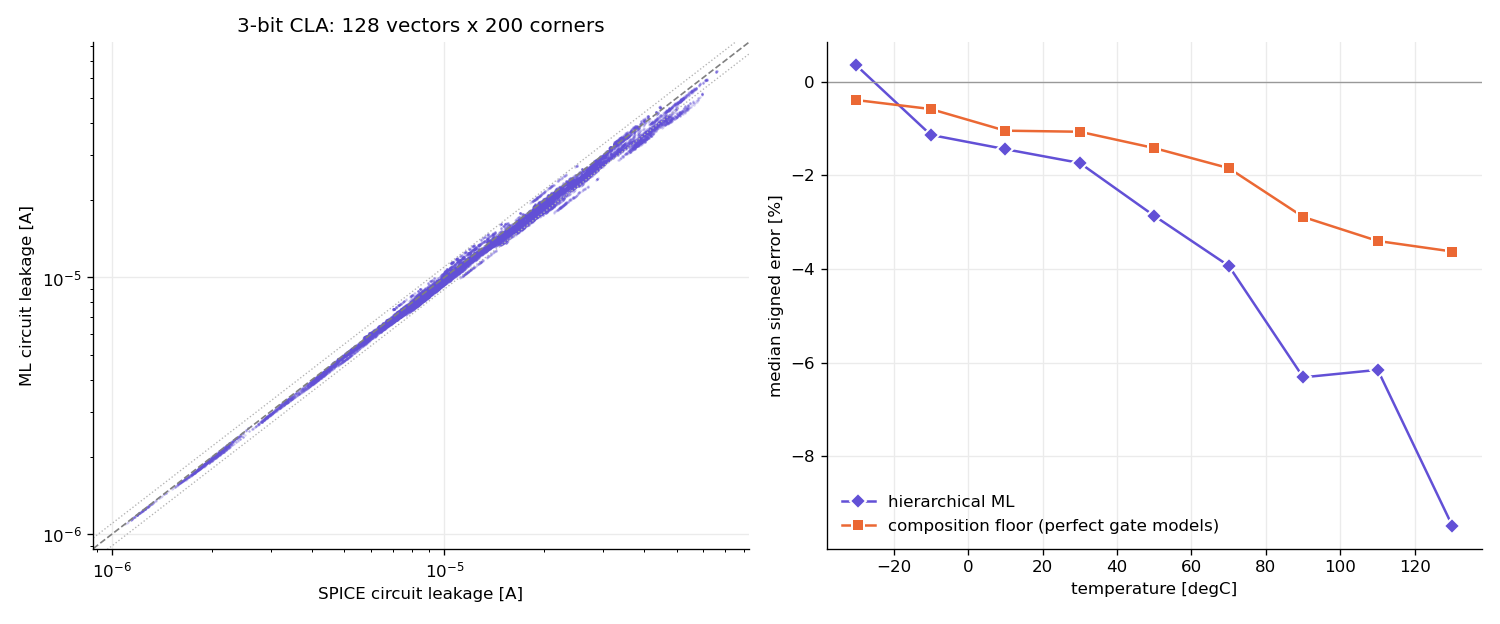
\includegraphics[width=0.9\textwidth]{circuit_parity.png}
\caption{Left: ML vs SPICE leakage of complete circuit (log axes); right: median signed error vs temperature.}\end{figure}

Per-vector median error varies little (1.04--2.10\% across 128 vectors in per-vector table).

\section{Error Analysis}

\subsection{Gate Level}
Gate-level error depends weakly on corner except at high temperature/VDD (hot bin larger median/p95); no consistent trend with $v_{th0}$ or $t_{oxe}$. Temperature dependence is partly explained by internal inverter inputs (AND2/OR2) moving away from rails. OFF-transistor channel terms dominate the gate error budget (PMOS OFF largest), while gate/body current terms contribute negligibly to total gate leakage error. Worst points are concentrated at hot corners and cases with non-rail internal nodes (e.g. AND2 01, OR2 00), consistent with exponential OFF leakage sensitivity to small gate-voltage deviations.

\begin{figure}[H]\centering
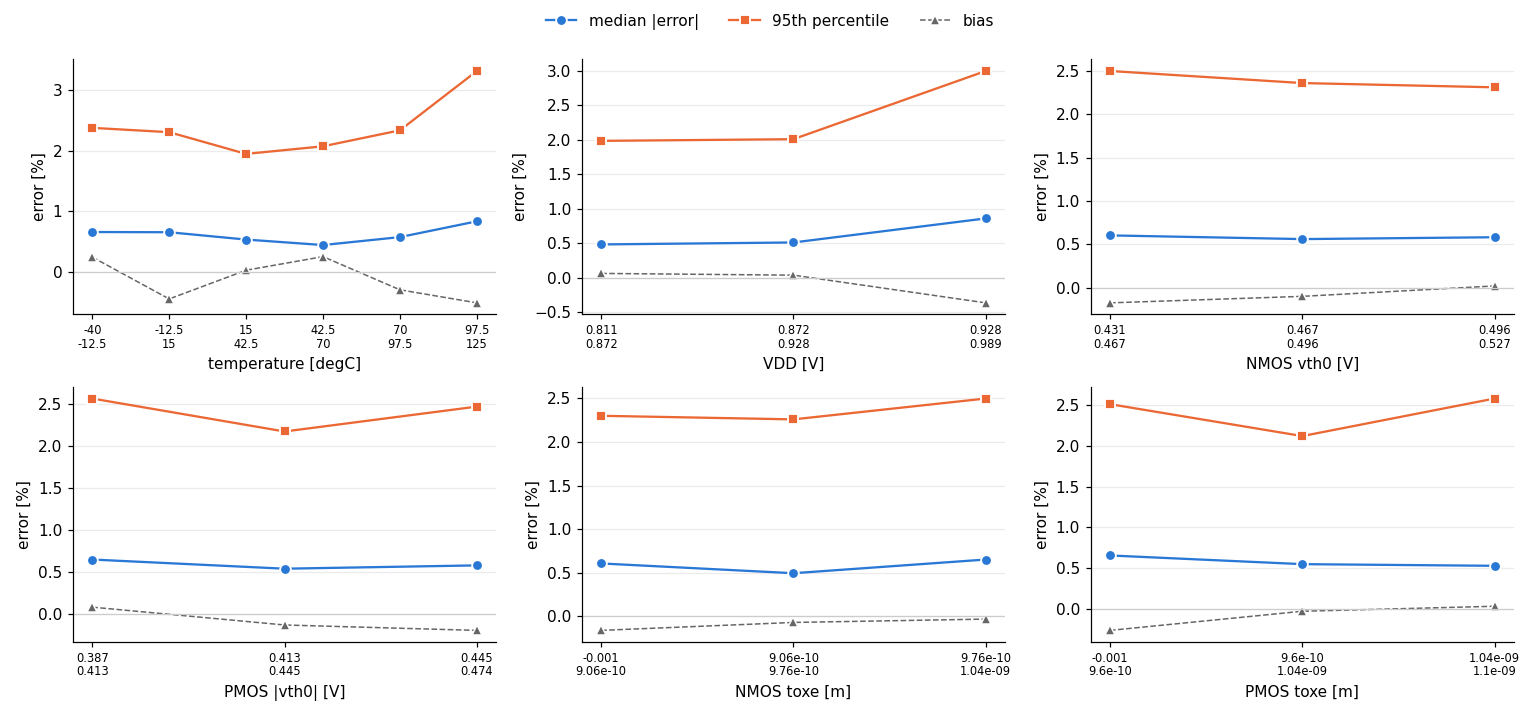
\includegraphics[width=0.9\textwidth]{gate_error_factors.png}
\caption{Gate-level error vs corner conditions (median, 95th percentile, bias).}\end{figure}

\subsection{Test Circuit}
Circuit-level error is strongly temperature-driven through composition: hierarchical and floor errors grow at hot corners while ML-vs-isolated-gate error remains comparatively small. Real gate inputs deviate from exact rails and outputs are loaded by downstream gates; both effects grow with leakage/temperature and are omitted by the prescribed hierarchical sum.

\section{Limitations and Improvements}
\begin{itemize}[leftmargin=*]
\item \textbf{Hierarchical composition / loading (main circuit shortfall).} Circuit prediction sums isolated-gate leakages with ideal 0/VDD inputs and no inter-gate loading (as prescribed). Composition floor is 1.37\% median / 5.25\% 95th / 1.85\% mean overall and worsens at hot corners (systematic underestimate), so 99\% circuit mean accuracy is not reachable there with this composition even with perfect gate models. \textbf{Simple improvement:} add a loading/voltage-propagation correction before summing gate leakages (estimate real gate output voltages and downstream input loading, or apply a first-order per-gate effective-load calibration).
\item \textbf{Non-rail gate inputs.} Internal inverter inputs in AND2/OR2 can be mV away from rails while models are trained/called at exact rails; OFF leakage is exponential in this deviation. Training with a small gate-voltage margin near rails would help.
\item \textbf{Training distribution vs operating region.} Gate operating points lie near $(V_d,V_s)$ corners at fixed $V_g,V_b$; uniform datasets are sparse there. Rail-sample refinement improved gate median/p95 substantially (1.49/7.36 $\to$ 0.58/2.37\%) with slight uniform-test tradeoff. Operating-region-aware sampling or active learning on gate-level error could improve further.
\item \textbf{Transistor accuracy.} PMOS OFF remains hardest (test median 1.28\%, p95 11.68\%), especially small/sign-sensitive currents and near data-resolution floor (4.4e-16 A). Large relative errors at very small $|V_{ds}|$ have limited gate impact.
\item \textbf{Leakage definition.} Project does not define gate leakage uniquely; supply-plus-input-power definition used (consistent with composition/KCL); supply-current-only differs materially only in specific cases (e.g. NOR2 11).
\item \textbf{Statistics/open points.} One split, one seed per model, 200 corners (no confidence intervals). Open: CLA includes Cin (7 inputs, 128 vectors used), acceptance of notebooks/scripts as code deliverable, and exact definition of ``mean accuracy'' (median/95th/mean relative errors all reported).
\end{itemize}

\section*{Contributions}
Work was divided across the team, with a slightly larger share to Lakshya Jindal and Sai Ritvik Uppuganti.
\begin{itemize}[leftmargin=*]
\item \textbf{Lakshya Jindal:} Led dataset generation and data-quality checks for the four transistor cases (sampling, SPICE runs, Kirchhoff/trend verification), and led transistor model development including preprocessing, training/comparison of model families, model selection, OFF-model refinement, and final model evaluation.
\item \textbf{Sai Ritvik Uppuganti:} Led development of the regeneration/testing workflow and self-contained scripts, gate-level and circuit-level validation runs, integration/debugging of the end-to-end pipeline, results verification, and report/LaTeX preparation and build support.
\item \textbf{Swarnava Pal:} Contributed to gate/corner setup and SPICE evaluation support, gate- and circuit-level analysis, plotting/result tabulation, documentation, and cross-checking of deliverables.
\item \textbf{Divesh Kumar:} Contributed to circuit-level validation and error analysis within the submitted project (SPICE/ML result comparisons, per-vector/corner checks, and supporting experiment runs), along with result cross-checking, debugging assistance, and documentation support.
\end{itemize}

\section*{Appendix A: Artifacts}
\begin{itemize}[leftmargin=*]
\item Datasets (4$\times$10k): \texttt{data/nmos\_on.csv}, \texttt{data/nmos\_off.csv}, \texttt{data/pmos\_on.csv}, \texttt{data/pmos\_off.csv}
\item Corners (200): \texttt{data/corners.csv} (common VDD/temp per corner; separate NMOS/PMOS process params \texttt{n\_*}, \texttt{p\_*})
\item OFF refinement extras (train/rail-val only): \texttt{data/extra\_nmos\_off.csv}, \texttt{data/extra\_pmos\_off.csv}
\item Netlists: \texttt{netlists/single\_*.cir} (4), \texttt{netlists/gate\_*.cir} (5), \texttt{netlists/test\_circuit\_cla3.cir}
\item Models: \texttt{models/nmos\_on.npz}, \texttt{models/nmos\_off.npz}, \texttt{models/pmos\_on.npz}, \texttt{models/pmos\_off.npz}
\item Key result tables: \texttt{results/model\_comparison\_table.csv}, \texttt{results/chosen\_models\_test.csv}, \texttt{results/final\_models\_test.csv}, \texttt{results/final\_models\_test\_per\_terminal.csv}, \texttt{results/gate\_results.csv}, \texttt{results/circuit\_results.csv}, \texttt{results/circuit\_results\_by\_vector.csv}, \texttt{results/refinement\_before\_after.csv}, \texttt{results/kirchhoff\_check.csv}, \texttt{results/trend\_check.csv}
\item Plots: \texttt{results/kirchhoff\_check.png}, \texttt{results/trend\_*.png}, \texttt{results/model\_comparison.png}, \texttt{results/pred\_vs\_spice\_*.png}, \texttt{results/gate\_parity.png}, \texttt{results/gate\_error\_factors.png}, \texttt{results/circuit\_parity.png}
\item Code (regenerate in order, fixed seeds): \texttt{scripts/01\_gen\_data.py}--\texttt{scripts/07\_error\_analysis.py}, \texttt{scripts/run\_all.py}; notebooks: \texttt{notebooks/01\_gen\_data.ipynb}--\texttt{notebooks/07\_error\_analysis.ipynb}
\end{itemize}

\end{document}
